\documentclass[titlepage,a4paper]{article}

\usepackage{a4wide}
\usepackage[colorlinks=true,linkcolor=black,urlcolor=blue,bookmarksopen=true]{hyperref}
\usepackage{bookmark}
\usepackage{fancyhdr}
\usepackage[spanish]{babel}
\usepackage[utf8]{inputenc}
\usepackage[T1]{fontenc}
\usepackage{graphicx}
\usepackage{float}

\pagestyle{fancy} % Encabezado y pie de página
\fancyhf{}
\fancyhead[L]{TP2 - Grupo 11}
\fancyhead[R]{Algoritmos y Programación III - FIUBA}
\renewcommand{\headrulewidth}{0.4pt}
\fancyfoot[C]{\thepage}
\renewcommand{\footrulewidth}{0.4pt}

\begin{document}
\begin{titlepage} % Carátula
	\hfill
\includegraphics[width=6cm]{logofiuba.jpg}
    \centering
    \vfill
    \Huge \textbf{Trabajo Práctico 2 — Java}
    \vskip2cm
    \Large [7507/9502] Algoritmos y Programación III\\
    Curso 2 \\ % Curso 1 para el de la tarde y 2 para el de la noche
    Segudo cuatrimestre de 2019 
    \vfill
    \begin{tabular}{ | l | l | l | } % Datos del alumno
      \hline \hline
      Alumno & Número de padrón & Email\\ \hline \hline
      CLAROS, ELVIS & 99879 & eclaros@fi.uba.ar\\ \hline
      BARRIO, HERNÁN & 89317 & hbarrio86@gmail.com\\ \hline
      MENDEZ, GABRIELA & 101741 & gabrielamendezg@outlook.com\\ \hline
      MARTINEZ, SELENE ANAHI & 100439 & zeluuh@gmail.com\\ \hline
    
  	\end{tabular}
    \vfill
    \vfill
\end{titlepage}

\tableofcontents % Índice general
\newpage

\section{Introducción}\label{sec:intro}
El presente informe reúne la documentación de la solución del segundo trabajo práctico de la materia Algoritmos y Programación III que consiste en desarrollar una aplicación de un Juego de Tablero con nombre \textbf{AlgoChess} en Java utilizando los conceptos del paradigma de la orientación a objetos vistos en el curso.

\section{Supuestos}\label{sec:supuestos}
% Deberá contener explicaciones de cada uno de los supuestos que el alumno haya tenido que adoptar a partir de situaciones que no estén contempladas en la especificación.

En el grupo una delas primeras interrogantes que surgió es, \textit{¿un jugador en su turno puede mover y/o atacar?}, nosotros para la resolución de este TP vamos a tomar la opción de \textbf{un jugador en su turno so lo va poder atacar o mover}.


\section{Diagramas de clase}\label{sec:diagramasdeclase}
% Uno o varios diagramas de clases mostrando las relaciones estáticas entre las clases.  Puede agregarse todo el texto necesario para aclarar y explicar su diseño. Recuerden que la idea de todo el documento es que quede documentado y entendible cómo está implementada la solución.

Nunc molestie facilisis diam in auctor. Nulla sed porta nibh, eu elementum erat. Vestibulum in lectus ornare, sollicitudin ipsum eget, posuere risus. Duis ac ante sagittis, ornare urna a, scelerisque purus. Orci varius natoque penatibus et magnis dis parturient montes, nascetur ridiculus mus. Ut commodo ultricies luctus. In a elit malesuada, semper felis at, varius lorem. Aenean hendrerit vitae lorem sit amet porttitor. Suspendisse vitae vulputate elit, a commodo lacus. Phasellus maximus arcu et eros sollicitudin, eu aliquet nulla efficitur. Aenean semper neque nec dignissim rutrum. Aliquam at purus vel tortor fringilla iaculis sit amet sit amet metus. Pellentesque faucibus a nulla eget molestie.

\begin{figure}[H]
\centering
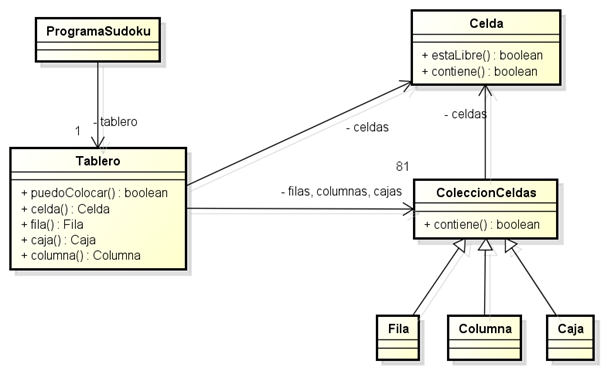
\includegraphics[width=0.8\textwidth]{DiagramasDeClases/diagrama_clase01.png}
\caption{\label{fig:class01}Diagrama del Sudoku.}
\end{figure}

\section{Diagramas de secuencia}\label{sec:diagramasdesecuencia}
% Mostrar las secuencias interesantes que hayan implementado. Pueden agregar texto para explicar si algo no queda claro.

Sed scelerisque est at augue finibus, at faucibus erat venenatis. Phasellus euismod magna mi, nec malesuada quam pretium id. Donec vel diam eleifend, lobortis leo nec, semper sapien. Nunc ultricies mauris augue, id iaculis erat vehicula in. Nam molestie metus vel mi tincidunt lacinia. Nunc a cursus nisl, id sollicitudin mauris. Donec sit amet condimentum dolor, eget rutrum augue.

\begin{figure}[H]
\centering
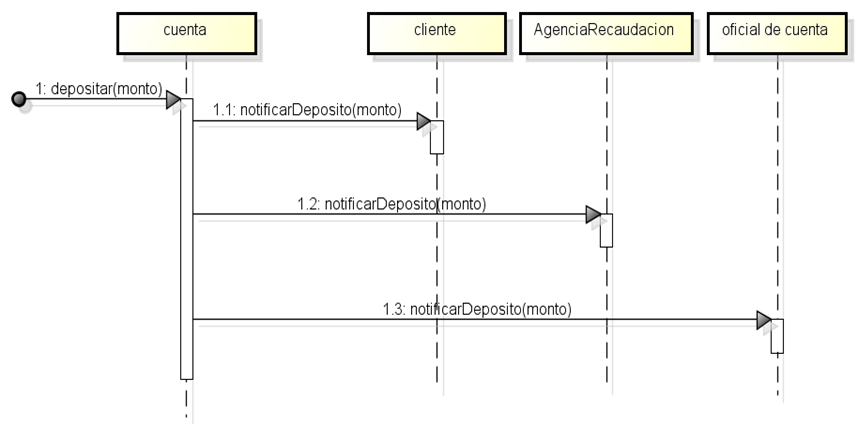
\includegraphics[width=0.8\textwidth]{DiagramasDeSecuencia/diagrama_secuencia01.png}
\caption{\label{fig:seq01}Aliquam rutrum justo sed.}
\end{figure}

Cras est velit, aliquet quis sagittis ornare, volutpat ac risus. Sed ullamcorper tellus orci, non viverra nulla rhoncus nec. Vivamus pretium dui pellentesque dolor molestie facilisis. Pellentesque tristique egestas magna quis tincidunt. Suspendisse non urna dolor. Fusce arcu erat, posuere in nibh at, gravida vulputate ligula. Ut erat erat, facilisis ac tristique eget, mattis sit amet nulla.

Sed ultrices pretium libero eget iaculis. Nulla facilisi. Suspendisse ornare, ligula vitae feugiat faucibus, nisi dolor ullamcorper urna, eu commodo lectus felis fermentum purus. Nunc vitae nunc nec dolor suscipit auctor. Curabitur euismod, leo non consequat congue, nibh ex aliquam urna, eget condimentum lectus urna venenatis magna. Praesent egestas sodales nibh, ut posuere ante vulputate sed. Vivamus gravida, orci sit amet auctor interdum, felis ipsum dapibus massa, sed commodo nisi risus ac nibh. Nunc ac viverra massa. Phasellus tempor arcu sapien, sit amet blandit velit bibendum non.

Duis est eros, laoreet viverra molestie ac, fringilla eget sapien. Sed molestie consequat sem non ultrices. Nulla sed velit nisl. Nunc luctus at neque et vehicula. Nulla feugiat velit in vestibulum rhoncus. Integer lobortis accumsan massa condimentum eleifend. Donec condimentum mauris sit amet purus bibendum, id bibendum odio pretium. Ut sollicitudin tellus vel nibh viverra, et aliquam ipsum iaculis. Duis tellus eros, sodales in aliquam vestibulum, porttitor tempus ipsum. Maecenas ac tincidunt nisl, et placerat leo. Fusce sit amet lectus nisl.

\begin{figure}[H]
\centering
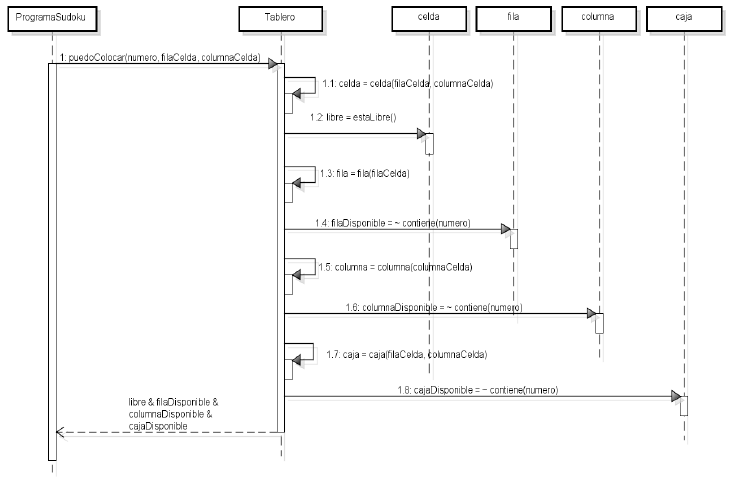
\includegraphics[width=\textwidth]{DiagramasDeSecuencia/diagrama_secuencia02.png}
\caption{\label{fig:seq02}Nam a nulla non mauris ullamcorper.}
\end{figure}

Donec efficitur, sapien quis consectetur bibendum, metus magna finibus metus, id venenatis dolor est eu tortor. Phasellus pellentesque, leo quis placerat ornare, sem purus porttitor enim, ac consectetur neque magna id ante. Donec tempor urna nisl, eget convallis elit aliquet sit amet. Phasellus turpis ex, malesuada vel tellus in, blandit suscipit diam. Vestibulum pulvinar leo a ornare laoreet. Vivamus volutpat velit dui, ac accumsan enim iaculis ac. Duis commodo a nulla et consectetur.

Sed sed diam in elit vulputate ultricies. Sed at felis mauris. Proin turpis est, sollicitudin ac arcu ac, blandit hendrerit est. Duis eu sagittis purus. Sed blandit dolor molestie justo sagittis pulvinar. Donec consequat urna at nunc finibus ullamcorper. Nam nulla nibh, vehicula id feugiat id, hendrerit a dolor. Vestibulum ante ipsum primis in faucibus orci luctus et ultrices posuere cubilia Curae; Fusce nec orci ut nibh convallis suscipit id sed est. Aenean placerat, est eget vehicula posuere, est eros pretium mi, sed porttitor nibh augue eget odio. Nulla mi lacus, placerat tincidunt magna non, suscipit lobortis urna.

Duis consequat varius sem, eu vehicula ex interdum quis. Integer consequat massa et fermentum tincidunt. Nam rutrum vestibulum nunc, eget tempus ex condimentum eget. Nunc id sollicitudin lectus. Vivamus porta sodales nisl nec tempor. Ut rhoncus accumsan sem eu consequat. Suspendisse eu metus a tellus convallis pharetra. Donec hendrerit, sapien a egestas iaculis, justo ante sodales elit, sed finibus ex purus a massa. Vivamus quis libero velit. Sed in ornare odio, ac facilisis magna. Donec rutrum orci ligula, nec interdum ipsum tristique ut. Vestibulum non orci finibus, hendrerit sem convallis, sagittis nunc. Aliquam vel laoreet dolor. Vivamus dignissim commodo magna, quis vestibulum libero aliquet nec. Praesent malesuada porta neque varius dictum.

\section{Diagrama de Paquetes}\label{sec:diagramadepaquetes}
% Incluir un diagrama de paquetes UML para mostrar el acoplamiento de su trabajo

Donec fermentum volutpat diam, non sodales dui pulvinar nec. Vestibulum eu nisl lacus. Maecenas vel tortor efficitur, volutpat nulla id, ornare sem. Quisque nisi magna, vulputate sed purus eget, elementum volutpat velit. Suspendisse sit amet feugiat nulla. Vivamus posuere sit amet diam condimentum sagittis. Sed et sapien in purus mattis ullamcorper sit amet non massa. Suspendisse tempus eleifend dapibus.

\section{Diagramas de Estado}\label{sec:diagramasdeestado}
% Incluir diagramas de estados, mostrando tanto los estados como las distintas transiciones para varias entidades del modelo.

Donec fermentum volutpat diam, non sodales dui pulvinar nec. Vestibulum eu nisl lacus. Maecenas vel tortor efficitur, volutpat nulla id, ornare sem. Quisque nisi magna, vulputate sed purus eget, elementum volutpat velit. Suspendisse sit amet feugiat nulla. Vivamus posuere sit amet diam condimentum sagittis. Sed et sapien in purus mattis ullamcorper sit amet non massa. Suspendisse tempus eleifend dapibus.

\section{Detalles de implementación}\label{sec:implementacion}
% Explicaciones sobre la implementación interna de algunas clases que consideren que puedan llegar a resultar interesantes.

\subsection{Tablero}
Esta clase ...

\begin{verbatim}
| rango |
rango := (2 to: 20) asOrderedCollection.
Transcript show: rango ; cr.
rango copy do: [ :unNumero | unNumero isPrime ifFalse: [ rango remove: unNumero ] ].
Transcript show: rango.
\end{verbatim}

\subsection{Jugador}
Jugador es una clase ...

\section{Excepciones}\label{sec:excepciones}
% Explicación de cada una de las excepciones creadas y con qué fin fueron creadas.

\begin{description}
\item[Exception] Lorem ipsum dolor sit amet, consectetur adipiscing elit. Proin nec facilisis odio. Pellentesque habitant morbi tristique senectus et netus et malesuada fames ac turpis egestas. In aliquam dapibus lacus at condimentum. Curabitur ornare scelerisque euismod. Duis a mi in nulla sodales sollicitudin vehicula sit amet sapien. Quisque vel eros ut libero consequat scelerisque. Nullam efficitur ante eu massa gravida sollicitudin.
\item[Excepcion] Curabitur elementum laoreet molestie. Ut hendrerit, quam lobortis porttitor cursus, ex sem facilisis massa, in interdum odio risus hendrerit dui.
\item[Excepcion] Integer porta efficitur felis. Etiam facilisis consectetur sem, ac efficitur orci. Nam a ante commodo, fringilla nisl a, sollicitudin est.
\item[Excepcion] Aliquam erat volutpat. Fusce quis efficitur augue. Fusce egestas mauris a nisi finibus volutpat. Maecenas venenatis ligula ut nisi maximus, vel ultricies enim scelerisque.
\item[Excepcion] Mauris gatis feugiat erat non euismod. Donec sagittis orci enim, et convallis lacus sodales at. Nunc laoreet leo vel metus eleifend, vel aliquam sem tincidunt. Nunc imperdiet eget erat eget tincidunt. Morbi tempus risus quis nulla faucibus facilisis. Sed varius nunc vel neque rutrum vestibulum.
\end{description}

\end{document}
